\documentclass{book}
\usepackage{amsmath, amssymb, amsthm}
\usepackage{geometry}
\usepackage[CJKspace]{xeCJK}  % 한글 지원
\setmainfont{Times New Roman}
\setCJKmainfont{Malgun Gothic}  % 시스템에 따라 다른 한글 글꼴 사용 가능

\usepackage{tikz}
\usepackage{pdflscape}
\usetikzlibrary{trees}

\geometry{
 a4paper,
 left=10mm,
 right=10mm,
 top=15mm,
 bottom=15mm
 }
 
 \setlength{\parindent}{0pt}

\title{낙서}
\author{사서림}
\date{2025.05.26.\text{\_\-\-\_}}

\begin{document}
\maketitle

\tableofcontents

\part{part}
\chapter{chapter}
\section{section}
\subsection{subsection}

\part{DBBD관련}

\chapter{DBBD관련 수식}
만약 가로 H, 세로 W인 이미지를 한번에 K개씩 각각 x,y축으로 분해한다면 최대 분해 가능한 깊이 M은 다음과 같다. (참고로 K는 x축 분활 갯수와 y분할 갯수의 곱이다. 즉 $K=\text{x축 분할 갯수}\times\text{y축 분할 갯수}$)
\[
M=\lceil \log_{K}HW \rceil
\]
이때 a를 의미 표현 보존률이라고 하면 a를 구하는 방법은 다음과 같다.
\[
M=\lceil \log_{K}aHW \rceil
\]
이때 올림을 제거하고 보면
\[
M=\log_{K}aHW
\]
에서 전개하면
\[
M=\log_{K}aHW=\log_{K}a+\log_{K}HW \rightarrow M-\log_{K}HW=\log_{K}a \rightarrow a=K^{M-\log_{K}HW}=\frac{K^M}{K^{\log_{K}HW}}=\frac{K^M}{HW}
\]
임으로 의미 표현 보존률 a는 다음과 같다.
\[
a=\frac{K^M}{HW}
\]
이때 a는 M의 최대 깊이로 HW 크기의 이미지일 시 최대 깊이로 이미지의 몇 \%를 유의미하게 분해할 수 있는지를 나타낸다. 이때 $\sqrt{a}\text{는}$ H, W에 각각 곱하면 100\%유의미하게 분해할 수 있는 비율이다.

이때 M의 최대 깊이 일시 a가 1인 $L \times L\text{크기인}$ 정사각형이 되는 L을 찾으면 다음과 같다.
\[
1=\frac{K^M}{L^2} \rightarrow L^2=K^M \rightarrow L=\sqrt{K^M}
\]
\newline\newline
그럼 이제 이것을 일반화 시켜서 $(\mathbb{R}^+)^n$에서의 분해를 살펴보자 만약 모든 각 차원을 k개로 분활한다면 $K=k^n$이다. 이때 M과 a 그리고 L에 관한 공식은 아래와 같다.
\[
\text{shape}=\{L_1, L_2, \ldots , L_n\}\text{일시}~~~~ ~~~~M=\left\lceil \log_{K}\left( \prod_{i=1}^n L_i \right) \right\rceil\text{임으로}~~~~ ~~~~M=\left\lceil \log_{k^n}\left( \prod_{i=1}^n L_i \right) \right\rceil \Rightarrow M=\left\lceil \frac{1}{n} \log_{k}\left( \prod_{i=1}^n L_i \right) \right\rceil
\]
\newline\newline
\[
a=\frac{K^M}{\prod_{i=1}^n L_i}=\frac{(k^n)^M}{\prod_{i=1}^n L_i}=\frac{k^{nM}}{\prod_{i=1}^n L_i}
\]
\newline\newline
\[
L^n=K^M \rightarrow L=\sqrt[n]{K^M}=\sqrt[n]{(k^n)^M}=\sqrt[n]{(k^M)^n}=k^M
\]

\newpage

이제 일반화 된 식들을 보자
\[
M=\left\lceil \frac{1}{n} \log_{k}\left( \prod_{i=1}^n L_i \right) \right\rceil~~~~ ~~~~
a=\frac{k^{nM}}{\prod_{i=1}^n L_i}~~~~ ~~~~~
L=k^M
\]
여기에서 $k=2$라고 해보자
\[
M=\left\lceil \frac{1}{n} \log_{2}\left( \prod_{i=1}^n L_i \right) \right\rceil~~~~ ~~~~
a=\frac{2^{nM}}{\prod_{i=1}^n L_i}~~~~ ~~~~~
L=2^M
\]
여기에서 시간축 T를 추가하여 가로 H, 세로 W인 동영상이 있다고 하자. 그럼 식은 아래와 같아진다.
\[
M=\left\lceil \frac{1}{3} \log_{2}\left( HWT \right) \right\rceil~~~~ ~~~~
a=\frac{2^{3M}}{HWT}=\frac{8^M}{HWT}~~~~ ~~~~~
L=2^M
\]
이때 만약 FHD급인 영상이 10분에 60Hz 짜리라고 해보자 그러면 $H=1920, W=1080, T=\text{fps}\times60\times10=60\times60\times10=36,000$이다. 그럼 이때 M을 구해보자.
\[
M=\left\lceil \frac{1}{3} \log_{2}\left( 1920 \times 1080 \times 36000 \right) \right\rceil=\left\lceil \frac{1}{3} \log_{2}\left( 74,649,600,000 \right) \right\rceil \approx \lceil 12.03980516 \rceil = 13
\]
그런대 시스템 상 최대 부하가 $M=10$이라고 하자 이때 이 동영상의 몇 \%를 유의미하게 분해할 수 있는지를 나타내는 a를 구해보자.
\[
a=\frac{8^10}{74,649,600,000} \approx 0.01438375857 \approx 0.0144 = 1.44[\%]
\]
무려 1\%정도만 유의미하다는 충격적인 결과가 나왔다. 그럼 이번에는 $M=12$라고 해보고 다시 계산해보자.
\[
a=\frac{8^12}{74,649,600,000} \approx 0.9205605487 \approx 0.9206 = 92.06[\%]
\]
이때는 90\%가 넘음으로써 정보를 충분히 생략하는 수준에 머문다. 그럼 3차원 데이터량 $Data_3=HWT$라고 할시 이를 모두 동일한 길이 L로 나누어 보자.
\[
L=\sqrt[3]{Data_3} \approx 4210.585543
\]
이때 $M=13$일때의 L과 비교해보자.
\[
L_\text{stand}=2^{13}=8192~~~~ ~~~~L \approx 4211~~~~ ~~~~ \frac{L_\text{stand}}{L} \approx 1.945381144621230111612443600095
\]
임을 알 수 있다.

\newpage

만약 DBBD를 이용해서 도트화처럼 하기 위하여 $M=\lceil \log_{K}(HW) \times 2^{-\frac{2}{3}} \rceil$로 M을 구하여 했다고 하자 그럼 $M=\lceil \log_{K}aHW \rceil$으로 바꾸어 a로 쓸 수 있는지에 대하여 알아보겠다. 간단히 알아보기 위하여 올림은 제거하고 보겠다. 그럼 아래와 같이 된다.
\[
M= \log_{K}(HW) \times 2^{-\frac{2}{3}}~~~~M=\log_{K}aHW \text{이므로}~~~~ \log_{K}(HW) \times 2^{-\frac{2}{3}}=\log_{K}aHW
\]
여기에서 a로 정리하면 다음과 같다.
\[
\log_{K}(HW) \times 2^{-\frac{2}{3}}=\log_{K}aHW=\log_{K}a+\log_{K}HW \Rightarrow \log_{K}(HW)\times2^{-\frac{2}{3}} - \log_{K}(HW) = \log_{K}a
\]
\[
\left( 2^{-\frac{2}{3}} - 1 \right) \log_{K}HW=\log_{K}a
\]
이때 $2^{-\frac{2}{3}}$를 도트 비율 조절 상수 $\tau$라고 하자 그럼 아래와 같이 바뀐다.
\[
\left( \tau - 1 \right) \log_{K}HW=\log_{K}a
\]
여기에서 정리하면
\[
a=K^{\left( \tau - 1 \right) \log_{K}HW}=\left( K^{\log_{K}HW} \right)^{\left( \tau - 1 \right)}=HW^{(\tau - 1)}
\]
그러므로 $\tau$에 대하여 a는 다음과 같다.
\[
a=HW^{(\tau - 1)}
\]
$\tau$를 구해보자
\[
\tau=1+\log_{HW}(a)
\]
\newline\newline
이번에는 한 깊이에서 최대로 생성 될 수 있는 블록의 수에 대한 공식을 말하겠다. 그 공식은 아래와 같다.
\[
\text{최대로 생성 될 수 있는 블록의 수}=K^M
\]
이때 하이퍼 트리의 개념을 적용하면 다음과 같다.
\[
\text{최대로 생성 될 수 있는 블록의 수}=\sum_{i=1}^M K^i
\]
그럼 이때 $M=10$일 때 일반 생성과 하이퍼 트리 생성을 비교하면 최대 깊이가 아닌 블록의 수를 구할 수 있다.
\[
\text{최대 깊이가 아닌 블록의 수}=\sum_{i=1}^M K^i - K^M = \sum_{i=1}^{M-1} K^i
\]
그럼 하이퍼 트리시 낭비 되는 메타 데이터(최대 깊이가 아닌 블록)의 비율을 구해보자.
\[
\text{하이퍼 트리에서 메타 데이터로 낭비 되는 블록의 비율}=\frac{\sum_{i=1}^{M-1} K^i}{\sum_{i=1}^M K^i}=\frac{\sum_{i=1}^{M-1} K^i}{K^M+\sum_{i=1}^{M-1} K^i}=1 - \frac{K^M}{K^M + \sum_{i=1}^{M-1} K^i}
\]
이때 $K=4, M=13$일시 발생하는 메타 데이터로 낭비 되는 비율은 $\frac{\sum_{i=1}^{12} 4^i}{\sum_{i=1}^{13} 4^i} \approx 24.99999888[\%]$임을 알 수 있다.
\newline\newline
이때 $K=4, M=1$일시 발생하는 메타 데이터로 낭비 되는 비율은 방금 구한 하이퍼 트리에서 메타 데이터로 낭비 되는 블록의 비율 공식으로 구하지 못한다. 그러나 애초에 낭비되는 블록이 하나도 없음을 알 수 있다.
\newline\newline
이때 $K=4, M=2$일시 발생하는 메타 데이터로 낭비 되는 비율은 $\frac{\sum_{i=1}^{1} 4^i}{\sum_{i=1}^{2} 4^i} = 20[\%]$임을 알 수 있다.
\newline\newline
이때 $K=4, M=100$일시 발생하는 메타 데이터로 낭비 되는 비율은 $\frac{\sum_{i=1}^{99} 4^i}{\sum_{i=1}^{100} 4^i} \approx 25[\%]$임을 알 수 있다.
\newline\newline
즉 일반적으로 전체 블록의 최대 $20[\%] \sim 25[\%]$의 블럭이 메타 데이터로 소모될 가능성이 있는 것이다.
\newline\newline
그럼 이때 M을 $\infty$로 보내보자. 그 결과는 아래와 같다.
\[
\lim_{M \to \infty}{ \frac{\sum_{i=1}^{M-1} K^i}{\sum_{i=1}^M K^i} }=\frac{1}{K}~~~~\text{if} \begin{pmatrix} \frac{1}{K} & K \end{pmatrix} \in \mathbb{R}^2 \land \log(K) > 0
\]
그럼으로 $K=4$일시 최대 25[\%]의 블록이 메타 데이터로 소모될 가능성이 있다고 볼 수 있다.

\newpage
\begin{landscape}
이번에는 이상적인 트리를 만들어보자. 루트(한번도 쪼게지지 않은 원본)주소를 0이라고 할시 규칙과 주소를 추적하는 법을 만들어보겠다.

아래는 $K=4, M=3$일시 이상적인 트리의 주소들이다.

\begin{center}
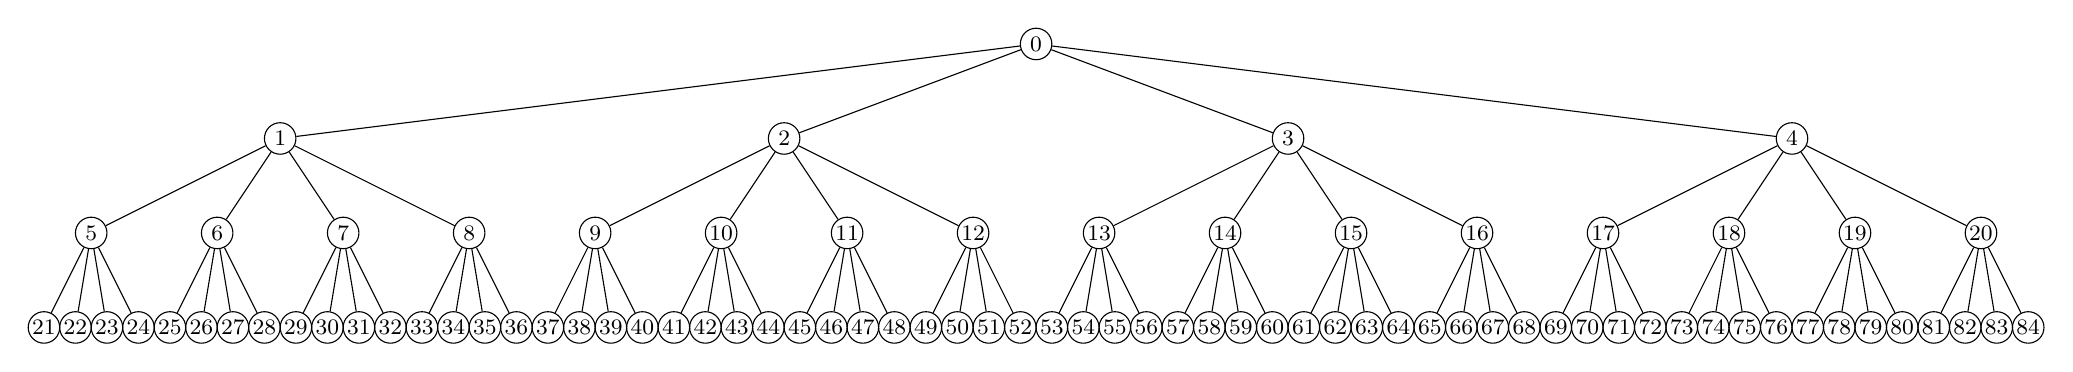
\begin{tikzpicture}[
  level 1/.style={sibling distance=64mm},
  level 2/.style={sibling distance=16mm},
  level 3/.style={sibling distance=4mm},
  level distance=12mm,
every node/.style={draw, circle, minimum size=4mm, inner sep=0pt, font=\footnotesize},
  edge from parent/.style={draw}
  ]

% 트리 정의
\node {0}
child {node {1}
    child {node {5}
        child {node {21}}
    	child {node {22}}
   	child {node {23}}
    	child {node {24}}}
    child {node {6}
        child {node {25}}
    	child {node {26}}
   	child {node {27}}
    	child {node {28}}}
    child {node {7}
        child {node {29}}
    	child {node {30}}
   	child {node {31}}
    	child {node {32}}}
    child {node {8}
        child {node {33}}
    	child {node {34}}
   	child {node {35}}
    	child {node {36}}}
  }
child {node {2}
    child {node {9}
        child {node {37}}
    	child {node {38}}
   	child {node {39}}
    	child {node {40}}}
    child {node {10}
        child {node {41}}
    	child {node {42}}
   	child {node {43}}
    	child {node {44}}}
    child {node {11}
        child {node {45}}
    	child {node {46}}
   	child {node {47}}
    	child {node {48}}}
    child {node {12}
        child {node {49}}
    	child {node {50}}
   	child {node {51}}
    	child {node {52}}}
  }
child {node {3}
    child {node {13}
        child {node {53}}
    	child {node {54}}
   	child {node {55}}
    	child {node {56}}}
    child {node {14}
        child {node {57}}
    	child {node {58}}
   	child {node {59}}
    	child {node {60}}}
    child {node {15}
        child {node {61}}
    	child {node {62}}
   	child {node {63}}
    	child {node {64}}}
    child {node {16}
        child {node {65}}
    	child {node {66}}
   	child {node {67}}
    	child {node {68}}}
  }
child {node {4}
    child {node {17}
        child {node {69}}
    	child {node {70}}
   	child {node {71}}
    	child {node {72}}}
    child {node {18}
        child {node {73}}
    	child {node {74}}
   	child {node {75}}
    	child {node {76}}}
    child {node {19}
        child {node {77}}
    	child {node {78}}
   	child {node {79}}
    	child {node {80}}}
    child {node {20}
        child {node {81}}
    	child {node {82}}
   	child {node {83}}
    	child {node {84}}}
};

\end{tikzpicture}

\vspace{1em}
\textbf{Figure: 트리 기반 블록 인덱스 시각화}
\end{center}

이 때 1번이 생성할 수 있는 주소는 45, 46, 47, 48번이다. 이를 유도하는 식을 세워 보자. 
11의 부모 주소는 2, 2의 부모 주소는 0이다. 이때 0은 깊이가 0, 2은 깊이가 1, 11은 깊이가 2이다. 이를 이용하여 구할 수 있다. 11의 위치는 깊이 1인 부모가 2번째이며, 깊이가 2인 본인이 $11 - \sum_{i=1}^{2-1} 4^i = 11 - 4 = 7$임으로 7번째임을 알 수 있다. 그럼 이때 7의 자식 주소 중 가장 낮은 주소는 $\sum_{i=1}^{3-1} 4^i + (7-1) \times \sum_{i=1}^{2-1} 4^i + 1=4+16+(7-1)\times4+1=20+24+1=45$임을 알 수 있다. 그리고 자식 주소 중 가장 높은 주소는 $\sum_{i=1}^{3-1} 4^i + 7 \times \sum_{i=1}^{2-1} 4^i=4+16+7\times4=20+28=48$임을 알 수 있다.
\newline\newline
그럼으로 D을 깊이, N을 현재 주소라고 하면 공식은 아래와 같다.
\[
\text{본인 노드가 같은 층에 있는 노드 중 몇 번째인지}=N - \sum_{i=1}^{D-1} 4^i
\]
\[
\text{본인 노드의 자식 노드 중 가장 낮은 주소}=1+\sum_{i=1}^{D} 4^i + 4 \left(-1 + N - \sum_{i=1}^{D-1} 4^i \right)
\]
\[
\text{본인 노드의 자식 노드 중 가장 높은 주소}=\sum_{i=1}^{D} 4^i + 4 \left(N - \sum_{i=1}^{D-1} 4^i \right)
\]
여기에서 K를 일반화 하면 아래와 같다.
\[
\text{본인 노드가 같은 층에 있는 노드 중 몇 번째인지}=N - \sum_{i=1}^{D-1} K^i
\]
\[
\text{본인 노드의 자식 노드 중 가장 낮은 주소}=1+\sum_{i=1}^{D} K^i + K \left(-1 + N - \sum_{i=1}^{D-1} K^i \right)
\]
\[
\text{본인 노드의 자식 노드 중 가장 높은 주소}=\sum_{i=1}^{D} K^i + K \left(N - \sum_{i=1}^{D-1} K^i \right)
\]

이때 47번의 부모를 구해보자. 47은 깊이가 3인것을 이미 알고 있다는 가정하에 다음과 같이 구할 수 있다. $\left \lceil \frac{N - \sum_{i=1}^{D-1} 4^i}{4} \right \rceil + \sum_{i=1}^{D-2} 4^i = \left \lceil \frac{47 - 4 - 16}{4} \right \rceil + 4 = \left \lceil \frac{27}{4} \right \rceil + 4 = \lceil 6.75 \rceil + 4= 7 + 4 = 11$임으로 11이 47의 부모이다.

\end{landscape}

그럼으로 D를 깊이, N을 현재 주소라고 하면 공식은 다음과 같다.
\[
\text{본인 노드가 같은 층에 있는 노드 중 몇 번째인지}=N - \sum_{i=1}^{D-1} K^i
\]
\[
\text{본인 노드의 자식 노드 중 가장 낮은 주소}=1+\sum_{i=1}^{D} K^i + K \left(-1 + N - \sum_{i=1}^{D-1} K^i \right)
\]
\[
\text{본인 노드의 자식 노드 중 가장 높은 주소}=\sum_{i=1}^{D} K^i + K \left(N - \sum_{i=1}^{D-1} K^i \right)
\]
\[
\text{본인 노드의 부모 노드의 주소}=\left \lceil \frac{N - \sum_{i=1}^{D-1} K^i}{K} \right \rceil + \sum_{i=1}^{D-2} K^i
\]
\[
\text{단}~\sum_{i=0}^{I} K^i, I < 0 \text{일시 그 부분은 0으로 처리해야 정합하게 돌아간다.}
\]
이 공식으로 이상적인 K진 트리를 만들어서 DBBD로 인한 유동적으로 자식 노드가 $1 \sim K$나올 시 저기에 K보다 자식 노드가 적을 시 자식 노드의 숫자 만큼 넣고 나머지는 빈공간으로 만드는 방식으로 정규화 시켜서 넣을 수 있게 되었다.

\newpage

$i$깊이에서 상위 깊이로 가는 식은 아래와 같다.
\[
s_{i+1}(x)=\left( \frac{W_i}{n}AB_i+b_i \right)
\]
\[
B_i \in \mathbb{R}^{n \times 15}~~\text{n개의 블록}~~~~
A \in \mathbb{R}^{1 \times n}~~\text{평균 벡터}~~~~
W_i \in \mathbb{R}~~\text{강도 조절}~~~~
\]
\[
b_i \in \mathbb{R}^{1 \times 15}~~\text{기준선 조절}~~~~
S \in \mathbb{R}^{15 \times 1}~~\text{의미 압축 벡터}~~~~
s_{i+1}(x) \in \mathbb{R}~~\text{하나의 스칼라 출력}
\]

\part{생성형 AI에 관한 나의 생각}

\chapter{공간에 관한 고찰}

ChatGPT 4o에 한번 랜덤한 프롬프트를 넣는다고 생각해보자. 여러분들은 어떤 프롬프트를 넣을 것인가? 그런대 이것을 자세하게 분석해보면 글, 그림이나 동영상, 파일을 넣을 수 있음을 알 수 있다. 이것을 이용하여 우리는 3가지 공간을 알 수 있다.
\[
T=\text{문자 공간}~~~~ ~~~~
M=\text{이미지-동영상 공간}~~~~ ~~~~
F=\text{파일 공간}
\]
이 때 T, M, F는 전체 공간 U에 속한다. 즉 $T, M, F \subset U$이다. 다만 U의 요소가 T, M, F만 있는 것은 아니며 더 다양하게 있을 수도 있으며 이는 어떻게 각각 하나의 의미 공간으로 묶어서 분류하느냐에 따라서 전체 공간의 구성이 달라질 수도 있음을 알린다.
\newline\newline
이때 컴퓨터에서 표현가능한 공간을 $B_R=\{0,1\}^\infty$라고 해보자 이때 컴퓨터는 무한을 표현할 수 없음으로 현실적으로 $B=\{0,1\}^n,~~n < \infty$임을 알 수 있다.

B와 U가 서로 손실 없이 상호 사상이 될 때 데이터를 온전히 다룰 수 있다. 즉 $U \Leftrightarrow B$이어야 한다. 그러므로 생성형 AI를 사상으로 표현하면 다음과 같다.
\[
\text{생성형AI} : U \rightarrow U
\]
그럼 다시 ChatGPT 4o로 돌아와서 $U=\{T,M,F\}$라고 하면 입력 가능한 공간은 일반적으로는 다음과 같다.
\[
\mathcal{P}(U) \setminus \phi = \{ \{ T,M,F \}, \{ T,M \}, \{ T, F \}, \{ M, F \},\{ T \}, \{ M \}, \{ F \} \}
\]
그럼 여기에서 그림 생성형 AI 사상을 만들어보자면 다음과 같다.
\[
m_k, m_{k+1} \subset M \text{이며}~ m_k \text{다음이}~ m_{k+1} \text{공간일 시}
\]
\[
\text{Transform} : m_k \rightarrow \{m_{k+1}, m_{k+1}, \ldots , m_{k+1}\} := m^m~~~~ ~~~~
\text{Group} : m^m \times \text{Condition} \rightarrow m_{k+1}
\]
그럼 이제 T, M, F공간이 실제로 각각 어떤 공간인지 알아보자
\[
T=\text{String 공간}~~~~ ~~~~
M=\text{Tensor 공간}~~~~ ~~~~
F=B\text{공간의 요소를 File해더에 따라 정의한 공간}
\]
이때 만약 T, M, F 서로 손실 없이 상호 사상이 되는 경우(또는 손실이 감당 가능할 정도로 적게 발생하면서 사상이 되는 경우) 즉 $T \Leftrightarrow M \Leftrightarrow F$일 시에는 T, M, F 공간 중 가장 유리한 공간에서 동작하는 모델로 돌려야 이득이다.

이제 M공간에서의 생성형 인공지능 정의를 U공간에서 생성하는 인공지능의 정의로 일반화 하면 다음과 같다.
\[
u_k, u_{k+1} \subset U \text{이며}~ u_k \text{다음이}~ u_{k+1} \text{공간일 시}
\]
\[
\text{Transform} : u_k \rightarrow \{u_{k+1}, u_{k+1}, \ldots , u_{k+1}\} := u^u~~~~ ~~~~
\text{Group} : u^u \times \text{Condition} \rightarrow u_{k+1}
\]
이때 LLM을 위한 Transformer를 CNN으로 구현하는 법을 생각해볼 수 있다. 즉 Transform사상의 결과인 $u^u$를 텐서 공간에서 각각의 유사도나 관계 등에 따라 $u^u$의 요소 각각의 텐서 공간안의 요소로 잘 정의하면 Attention을 정의하지 않아도 자연스럽게 Attention이 텐서 공간안에서 요소와 요소사이의 거리같은 것으로 구해질 가능성이 있다고 볼 수 있다.

\part{함수공간의 요소 W,b를 이용한 생성형 MLP 이론}
\chapter{블록 분해 기법에 관한 고찰}
\chapter{하이퍼 트리}

하이퍼 트리의 구조

1. 모든 노드에 데이터 값을 가진다.

2. 데이터 값은 Object나 추상 클래스 상속을 받아서 모든 데이터 유형을 리스트로 관리한다.

2.1. 또는 더욱 복잡한 버전으로는 List의 요소 각각을 하나의 데이터 값 유형을 가지는 하위 List로 가지게 하여 만든다.

3. 이 구조는 그래프의 업그래이드 버전이다.(자동 미분 처럼 모든 데이터 유형을 List나 List.List에 저장할 때 추상클래스로 한번 덮고 요소로 넣어야 할 것 같다.)

4. 쉽게 생각해서 이 자료구조는 이런 것이다. 차트나 전이 함수를 생각해보고 한 다양체에서 한 열린공간에서 다른 열린 공간으로 갈 때에는 그냥 선형적으로 기억해도 되며 그를 이용하여 전개할 수 있다. 한마디로 추상화된 선형공간인 것이다. 그와 같이 하이퍼 트리 자료구조 또한 선형성을 추상적으로 가지고 있다고 볼 수 있다. 그래서 다른 이름으로는 '선형 하이퍼 트리'라고 한다.

5. 엣지 또한 노드와 같은 구조이다.

\chapter{생성형 MLP 이론}
퍼셉트론은 $F:\mathbb{R}^2 \rightarrow \mathbb{N}_0$에서 $F:\mathbb{R}^n \rightarrow \mathbb{N}_0$, $F:\mathbb{R}^n \rightarrow (\mathbb{N}_0)^m$, $F:\mathbb{R}^n \rightarrow \mathbb{R}^m$의 형식으로 발전해왔다. 
\newline\newline
하나의 퍼셉트론(하나의 노드)를 $F:\mathbb{R}^n \rightarrow \mathbb{R}$라고 하자. 그럼 F들의 결과를 쌓은 것은 선형함수를 $L:\mathbb{R}^n->\mathbb{R}^m$ 비선형 함수를 $Q:\mathbb{R}^m->\mathbb{R}^m$라고 할때 그렇다면 한 층의 모든 노드에 관한 식은 $Q(L(x))$이다. 그리고 순전파는 $Q(L(Q(L(Q(L(\ldots))))))=M(x)$이다. $X \rightarrow Y$(모델에서의 입력->출력)으로 가는 정제된 해석은 대부분 벡터장이다.(모든 모델의 본질은 $M:X \rightarrow Y$이라는 사상이며, 이때 모델은 입력 공간 $X$ 위에 정의된 벡터장처럼 동작한다.)
\newline\newline
파라미터 $W,b$를 입력공간 $X$의 위상적 특징이 있는 상위 공간 $K$이며 미분 가능한 함수 공간의 요소라고 하자. 그럼 우리는 이를 아래와 같이 표현 가능하다.
\[
W \subset C^k(X, K),~~~~ X \subseteq K \subseteq \mathbb{R}^{n \times m}
\]
\[
b \subset C^k(X, K),~~~~ X \subseteq K \subseteq \mathbb{R}^{n}
\]

여기에서 BDDB를 이용하여 블럭 포함 여부에 따라 0, 1을 부여하는 함수 $\Omega_i(x)$을 이용한 베이시스 함수를 쓰면 아래와 같다
\[
W_{ij}(x) = \sum_{k = 1}^{k_\text{end}} \Omega_{ij}(x) \alpha_{ij} \phi_k(x;\beta_k) ~~~~ W(x)=\sum_{i=1}^{n} \sum_{j=1}^{m} W_{ij}(x) e_{ij}
\]
\[
b_{i}(x) = \sum_{k = 1}^{k_\text{end}} \Omega_{i}(x) \alpha_{i} \phi_k(x;\beta_k) ~~~~ b(x)=\sum_{i=1}^{n} W_{i}(x) e_{i}
\]
그리고 이때 베이시스 함수가 푸리에 급수라면 아래와 같다.
\[
W_{ij}(x) = \sum_{k = 1}^{k_\text{end}} \Omega_{ij}(x) \left( \beta_{k-\sin} \sin(k \omega t) + \beta_{k-\cos} \cos(k \omega t) \right) ~~~~ W(x)=\sum_{i=1}^{n} \sum_{j=1}^{m} W_{ij}(x) e_{ij}
\]
\[
b_{i}(x) = \sum_{k = 1}^{k_\text{end}} \Omega_{i}(x) \left( \beta_{k-\sin} \sin(k \omega t) + \beta_{k-\cos} \cos(k \omega t) \right)) ~~~~ b(x)=\sum_{i=1}^{n} W_{i}(x) e_{i}
\]

$\mathcal{L}$를 변분 손실함수라고 하자. 오차 하강법을 $P$를 $W,b$파라미터들을 모은 벡터 공간의 요소, $M(x)$를 MLP 순전파라고 하면 $P_{i+1} = P_i - \text{control}(P_i, \mathcal{L}, M, x) \delta P(\mathcal{L};n(x))$ 라고 하자. 변분 손실함수는 아래와 같다.
\[
\mathcal{L}(M)=\int_{X} \lVert M(x;W(x),b(x)) - y(x) \rVert dx
\]

여기에서 $P$는 $P=[W_1,b_1,W_2,b_2,\ldots,W_i,b_i]$인 벡터공간의 요소이다. 즉 우리는 여태 것 $W,b$파라미터의 집합으로 본 것을 벡터공간의 한 점 $P$로 봄으로서 학습 정도를 벡터 공간에서의 변화로 이해 할 수 있을 것이다. 이때 만약 $W,b$가 함수공간의 요소일 시 $P$는 $W,b$ 각각의 파라미터 $\alpha_{ij}, \alpha_{i}, \beta_k$ 묶음이다.

\part{또 다른 생각의 낙서}

\chapter{F분해 기법 - Generalized Functional Decomposition}
[F분해 기법 기본]

AI의 전처리를 위한 F분해 기법(Generalized Functional Decomposition)을 제안한다.

원함수 $F:\mathbb{R}^n \rightarrow \mathbb{R}^m$이며 정의역의 부분 공간 $D_i \subseteq \mathbb{R}^n$이고

근사함수 $f_i:D_i \rightarrow \mathbb{R}^m~,~f_{ik}:D_i \rightarrow \mathbb{R}~(\mathbb{R}^m\text{에서 k번째 차원 출력})$이며

스칼라장화 한 벡터장 원함수$F_k:\mathbb{R}^n \rightarrow \mathbb{R}~(\mathbb{R}^m\text{에서 k번째 차원 출력})$일시
\[
f_i\text{의 전체 정확도}~a(f_i) = \left ( 1 + \sum_{k=1}^m \int_{D_i} \lVert \nabla F_k(x) - \nabla f_{ik}(x) \rVert d \mathbf{x} \right )^{-1}
\]
\[
f_i\text{의 j정의역 차원에서의 1차원 정확도}~a_j(f_i) = \left ( 1 + \sum_{k=1}^m \int_{D_i \setminus X_j} \int_{X_j} \left \lVert \frac{\partial F_k(x)}{\partial x_j} - \frac{\partial f_{ik}(x)}{\partial x_j} \right \rVert dX_j d\mathbf{X} \right )^{-1}
\]
이 정확도들을 이용하여 F를 정확도에 미달하는 축이나 전체 축에 대하여 분활한다. 즉 해당 함수의 정의역 공간을 내밷는 함수(여기에서 분해는 [a,b]형태로 된다.)가 $D(F)=(D_x(F),D_y(F))=[D_{xs}(F),D_{xe}(F)] \times [D_{ys}(F),D_{ye}(F)]$일시 $F:\mathbb{R}^2 \rightarrow \mathbb{R}^3$에 대하여 임계값이 $\alpha$이고 미달하는 축에 대하여 2분할시 다음과 같이 나눠진다.
\[
P(F)=
\begin{cases}
\begin{matrix}
f_i: [D_{xs}(F),\frac{D_{xe}(F)}{2}] \times [D_{ys}(F),\frac{D_{ye}(F)}{2}]\rightarrow \mathbb{R}^3 \\
f_j: [\frac{D_{xe}(F)}{2},D_{xe}(F)] \times [D_{ys}(F),\frac{D_{ye}(F)}{2}]\rightarrow \mathbb{R}^3 \\
f_k: [D_{xs}(F),\frac{D_{xe}(F)}{2}] \times [\frac{D_{ye}(F)}{2},D_{ye}(F)]\rightarrow \mathbb{R}^3 \\
f_h: [\frac{D_{xe}(F)}{2},D_{xe}(F)] \times [\frac{D_{ye}(F)}{2},D_{ye}(F)]\rightarrow \mathbb{R}^3
\end{matrix} & \text{if}~ a(F) < \alpha \lor (a_x(F) < \alpha \land a_y(F) < \alpha) \\
\begin{matrix}
f_i:[D_{xs}(F),\frac{D_{xe}(F)}{2}] \times [D_{ys}(F),D_{ye}(F)] \rightarrow \mathbb{R}^3 \\
f_j:[\frac{D_{xe}(F)}{2},D_{xe}(F)] \times [D_{ys}(F),D_{ye}(F)] \rightarrow \mathbb{R}^3
\end{matrix} & \text{if}~ a_x(F) < \alpha \\
\begin{matrix}
f_i:[D_{xs}(F),D_{xe}(F)] \times [D_{ys}(F),\frac{D_{ye}(F)}{2}] \rightarrow \mathbb{R}^3 \\
f_j:[D_{xs}(F),D_{xe}(F)] \times [\frac{D_{ye}(F)}{2},D_{ye}(F)] \rightarrow \mathbb{R}^3
\end{matrix} & \text{if}~ a_y(F) < \alpha \\
F & \text{otherwise}\\
\end{cases}
\]

이를 $F$나 $f_i$들의 $P$에서의 출력이 전부 자기자신이 될 때까지 각각 반복한다.

이 때 각각 $D_i$에서 정의된 $f_i$들은 다음과 같이 선형 함수로 정의한다.

(이는 대표적인 근사 함수일 뿐 꼭 이걸로 해야한다는 것이 아니다.)
\[
f_i(x,y)=f_{ix}(x)+f_{iy}(y)
\]
\[
f_{ix}(x)=\frac{F(D_{xe}(f_i))-F(D_{xs}(f_i))}{D_{xe}(f_i)-D_{xs}(f_i)}x+F(D_{xs}(f_i))~~~~ ~~~~f_{iy}(y)=\frac{F(D_{ye}(f_i))-F(D_{ys}(f_i))}{D_{ye}(f_i)-D_{ys}(f_i)}y+F(D_{ys}(f_i))
\]

그럼으로 다음과 같이 결과가 나온다.\\
\[
F \approx \bigcup_{i} f_i~~~~ ~~~~\bigcup_{i \neq j} f_i \cap f_j = A \neq \phi
\]
이 때 $A$공간에서 $f_i$에서 $f_j$로 이동이 발생할 때 경계에서의 값을 다음과 같이 하도록 하자.
\[
T_{i \rightarrow j}(x):=T_{ij}(x)=f_j(x)-f_i(x)~~~~ ~~~~V:A \rightarrow T_{ij}(A) \rightarrow \mathbb{R}^m
\]
이렇게 하면$V$는 $f_i$들간 이동이 발생할 때의 순간 다차원 공역의 값 변화를 상대적으로 표현할 수 있다.

이 때 $V$를 이용하여 보자
\[
f_{Vij}(D_i \cap D_j \subseteq A )=V(A)(\mathbf{x} - \min (D(f_i)))+\frac{f_i(A)+f_j(A)}{2}
\]\\

[정확도 응용]

원함수 $F:\mathbb{R}^n \rightarrow \mathbb{R}^m$가 $F \in C^h$로 속한다고 하자.

그리고 $\nabla$를 h번 중첩 한 것을 여기에서는 다음과 같이 적어보기로 한다. $\nabla^hF:=\underbrace{\nabla(\nabla( \cdots \nabla(F) \cdots ))}_{\nabla\text{가 h번 중첩되어 있다}}~~~~\nabla^0F:=F$

그리고 또한 편미분에서 다음과 같은 상황을 이렇게 적어보기로 한다. $\frac{\partial^0 F(x)}{\partial x_j^0}:=F$

이 때의 $C^h$에 관한 정확도는 아래와 같이 정의하며 근사 함수 또한 $f \in C^h$로 속해야만 한다.

\[
f_i\text{의}~C^h\text{에 관한 전체 정확도}~H(f_i) = \left ( 1 + \sum_{k=1}^m \int_{D_i} \lVert \nabla^h F_k(x) - \nabla^h f_{ik}(x) \rVert d \mathbf{x} \right )^{-1}
\]
\[
f_i\text{의}~C^h\text{에 관한 j정의역 차원에서의 1차원 정확도}~H_j(f_i) = \left ( 1 + \sum_{k=1}^m \int_{D_i \setminus X_j} \int_{X_j} \left \lVert \frac{\partial^h F_k(x)}{\partial x_j^h} - \frac{\partial^h f_{ik}(x)}{\partial x_j^h} \right \rVert dX_j d\mathbf{X} \right )^{-1}
\]\\

그리고 모든 $0 \le z \le h,~~ C^z$에 대하여 검토하는 누적 정확도는 다음과 같다.

\[
f_i\text{의}~C^h\text{에 관한 전체 누적 정확도}~Z(f_i) = \left ( 1 + \sum_{k=1}^m \sum_{z=0}^h \int_{D_i} \lVert \nabla^z F_k(x) - \nabla^z f_{ik}(x) \rVert d \mathbf{x} \right )^{-1}
\]
\[
f_i\text{의}~C^h\text{에 관한 j정의역 차원에서의 1차원 누적 정확도}~Z_j(f_i) = \left ( 1 + \sum_{k=1}^m \sum_{z=0}^h \int_{D_i \setminus X_j} \int_{X_j} \left \lVert \frac{\partial^z F_k(x)}{\partial x_j^z} - \frac{\partial^z f_{ik}(x)}{\partial x_j^z} \right \rVert dX_j d\mathbf{X} \right )^{-1}
\]

여기에서 $z=0$일 때 전체 누적 정확도와 1차원 누적 정확도는 적분하는 순서만 바뀐 정확도임을 알 수 있다. 그리고 $2 \le h$일 경우 연산자 $H$, $H_j$, $Z$, $Z_j$에 대해서는 알아서 랭크-h 텐서에서의 노름을 잘 가져다가 쓰던가 정의해서 쓰기를 바란다.\\

다음으로 벡터장인 원함수 $\mathbf{F}$와 부분 정의역 $D_i$에서 정의된 벡터장인 근사 함수 $\mathbf{f}$에 대하여 강제로 스칼라장으로 나누지 않고 벡터장을 보존하면서 정확도를 구하는 벡터장 정확도는 다음과 같다.

\[
\mathbf{f}\text{의}~C^h\text{에 관한 벡터장 누적 정확도}~\tau(\mathbf{f}) = \left ( 1 + \sum_{z=0}^h \int_{D_i} \lVert \nabla^z \mathbf{F}(x) - \nabla^z \mathbf{f}(x) \rVert d \mathbf{x} \right )^{-1}
\]\\

다음으로 그로모프-하우스도르프 거리를 이용하여 정확도를 다음과 같이 구해보자. 이를 이용하여 정확도를 정의하는 법을 설명해보겠다. 원함수 $\mathbf{F}$를 다양체로 보고 부분 정의역 $D_i$에서의 부분 다양체 $\mathcal{M}$이 있다고 하자. 마찬가지로 부분 정의역 $D_i$에서 정의된 근사 함수 $\mathbf{f}$를 다양체로 보고 그를 유클리드 공간으로 근사한 $\mathbf{p}$가 있다고 한다. 이 때 $D_i$에서 $\mathcal{M}$과 $\mathbf{p}$의 그로모프-하우스도르프 거리를 $\mathbf{r}=d_{GH}(\mathcal{M},\mathbf{p})$라고 하면 정확도 $\tau_{GH}$는 다음과 같다.

\[
\mathbf{f}\text{의 그로모프-하우스도르프 거리를 이용한 정확도}~\tau_{GH}(\mathbf{f})= \left ( 1 + \mathbf{r} \right )^{-1}
\]\\

그리고 본 정확도들은 다 형태가 $1/(1 + \text{error})$ 꼴로 이루어져있는데 여기에서 $\text{error}$만 취하면 AI에서 쓸 수 있는 Loss Function이 된다.
또한 참고로 각 정확도 연산자의 이름으로 정한 이유는 각각 아래와 같다.

\[
a := \text{accuracy}
\]
\[
H := \text{Hessian}
\]
\[
Z := \text{Laplace transform에서의 complex}~z
\]
\[
\tau := \text{Topological}
\]
\[
\tau_{GH} := \text{Gromov-Hausdorff distance}
\]

\chapter{문양}
$z(t) = \left( t^{2.25} \cos(t) + t^2 \sin(9t^{1.75}) i \right) \times \exp \left( \frac{\pi t^{1.5}}{16} i \right)$

$A \xleftarrow{n+\mu-1} B \xrightarrow[T]{n\pm i-1} C$\\\newline

\begin{landscape}
\chapter{AI 모델}

일반적인 AI는 아래와 같이 정의된다.\\
$AI:(X:\mathbb{R}^n\rightarrow\mathbb{R}^m) \xrightarrow[\text{다양체가 포함된 사상}]{\mathcal{M}:X\rightarrow Y} (Y:\mathbb{R}^h\rightarrow\mathbb{R}^k)$\\
단 실질적으로는 사용자가 조절 할 수 없는 const 공간들이 있는 $X:=\mathcal{F}(\text{const}_x,R^m),~~ Y:=\mathcal{F}(\text{const}_y,R^k)$인 함수 공간이다. 이는 단순히 const의 공간의 기수가 크거나 작음이 문제가 아닌 const공간을 벗어나는 입력에 관하여 제대로 된 출력을 보장할 수 없다는 것을 의미한다.\\

내가 제안하는 AI모델(FDT - Functional Decomposition Transformer)의 흐름은 아래와 같다.\\
$M:(X:\mathbb{R}^n\rightarrow\mathbb{R}^m) \xrightarrow[\text{F분해 기법}]{} ((X:\mathbb{R}^n\rightarrow\mathbb{R}^m), F) \xrightarrow[f_i\text{트리 구조화 및 각 깊이마다 깊이 요약 그리고 상위 깊이만 존제할 경우 강제 분해 후 Latent Vector를 모든 노드에 대하여 생성한 Latent Matrix 생성}]{} \mathbb{R}^{r \times c} \xrightarrow[\mathbb{R}^{r \times c}\text{트리화}]{} \text{AI Model 사용하며 대표적으로는 Graph Transformer} \xrightarrow[\text{AI 모델 안에서의 사상}]{} (Y:\mathbb{R}^h\rightarrow\mathbb{R}^k)$

이때 $F:=\{f_1, f_2 ,\cdots, f_i\}=\{(f_1:D_1\rightarrow \mathbb{R}^m),(f_2:D_2\rightarrow \mathbb{R}^m), \cdots (f_i:D_i\rightarrow \mathbb{R}^m)\} \text{이다.}$

그리고 FDT에서는 사용자가 조절할 수 없는 const가 없거나 최대한 적게 만들 예정이다.\\

그럼 흐름을 한번 자세하게 보도록하겠다.\\

처음에는 5개의 공간에 대하여 논하고 그 다음에는 4개의 사상에 관하여 논하겠다. 이 중 F분해 기법은 이미 앞장에서 다뤘음으로 생략하기로 한다.\\\newline

1. $X:\mathbb{R}^n \rightarrow \mathbb{R}^m$ 공간과 $Y:\mathbb{R}^h\rightarrow\mathbb{R}^k$공간\\
- 본 공간은 $\mathcal{F}(\mathbb{R}^n, \mathbb{R}^m)$인 함수 공간이다. 다만 컴퓨터의 조밀성 구현 불능 한계로 인하여 실제로는 아래의 공간을 이용하도록 한다. 
float x bit 자료구조를 $\mathbb{Q}_{\text{float x bit}}:=\mathbb{Q}_{\text{float}}$라고 정의하면 컴퓨터에서는 다음 공간을 쓰며, 이때 float x bit 자료구조를 공간으로 표기할 때 IEEE 754표준에서 정의된 x bit인 float에 대하여는 그를 준수하여 공간의 기수와 성질을 정의하여야만 한다.\\
$X:\mathbb{N}_0^n \rightarrow \mathbb{Q}_{\text{float}}^m ~:=~ \mathcal{F}(\mathbb{N}_0^n , \mathbb{Q}_{\text{float}}^m)$\\\newline
근대 그렇다면 어떻게 현실세계의 $\mathcal{F}(\mathbb{R}^n, \mathbb{R}^m)$인 데이터를 $\mathcal{F}(\mathbb{N}_0^n , \mathbb{Q}_{\text{float}}^m)$로 제대로 변환할 수 있는가도 매우 중요할 것이다. 
이때 표본화(Sampling)라는 정의역 이산화 함수 공간$\mathcal{F}(\mathbb{R}^n,\mathbb{N}_0^n)$의 요소인 표본화 함수를 이용하여 정의역을 이산화 하고, 양자화(Quantization)라는 치역 이산화 함수 공간$\mathcal{F}(\mathbb{R}^m,\mathbb{Q}_{\text{float}}^m)$의 요소인 양자화 함수를 이용하여 치역을 이산화 하여야 한다.\\\newline
그런가 하면 반대로 어떻게 컴퓨터 세계의 $\mathcal{F}(\mathbb{N}_0^n , \mathbb{Q}_{\text{float}}^m)$인 데이터를 $\mathcal{F}(\mathbb{R}^n, \mathbb{R}^m)$로 제대로 변환할 수 있는가도 매우 중요할 것이다. 
이는 $\mathcal{F}(\mathbb{R}^n,\mathbb{N}_0^n)$의 요소인 표본화 함수를 $S$라고 하면 그에 대한 역사상 $S^{-1}$가 존재하며, $\mathcal{F}(\mathbb{R}^m,\mathbb{Q}_{\text{float}}^m)$의 요소인 양자화 함수를 $Q$라고 하면 그에 대한 역사상 $Q^{-1}$가 존재하여야 조밀한 현실세계로 무의미한 변환이라도 시도 가능함을 알 수 있다. 하지만 수학적으로 $S^{-1}$와  $Q^{-1}$는 존재하지 않는다. 그럼으로 $S^{-1}$와  $Q^{-1}$는 추론적으로 보간하는 함수이지 역사상이 아님을 강력하게 유의하여야만 하며 이 과정에서 원 공간$X:\mathbb{R}^n \rightarrow \mathbb{R}^m$에서의 원요소와 다른 요소를 가지게 될 수 있음을 기억하여야만 한다.\\

2. $((X:\mathbb{R}^n \rightarrow \mathbb{R}^m),F)$ 공간과 트리화 그리고 $\mathbb{R}^{r \times c}$공간\\
- 본 공간은 $\mathcal{F}(\mathbb{R}^n, \mathbb{R}^m)$과 F분해의 과정과 결과를 같이 모은 집합인 $F:=\{f_1, f_2 ,\cdots, f_i\}=\{(f_1:D_1\rightarrow \mathbb{R}^m),(f_2:D_2\rightarrow \mathbb{R}^m), \cdots (f_i:D_i\rightarrow \mathbb{R}^m)\}$의 순서쌍이다. 이 공간을 순서쌍으로 만든 이유는 원 공간 $X$와 $X$에 대해 분석한 공간 $F$를 $(X,F)$로 놓음으로써 위상공간의 $(X,\tau)$와 같이 어떤 공간 $X$와 그에 대한 위상 $\tau$를 놓는 것과 비슷한 흐름으로 읽히게 하기 위함이다.\\

그리고 F 집합 안의 $f_i$들의 밑 첨자인 숫자 i는 f의 F분해 시 DBBD(Depth-Based Binary Division)식으로 정의된 ID이다. 이 때 $(X,F)$공간의 F를 트리화 시키기 위하여 다음과 같이 정의한다.\\
집합 F의 한 요소 $f_i$가 말단노드이다. $\Longleftrightarrow$ F안의 $D_j \subset D_i$이고 $D_j \neq D_i$을 만족하는 다른 요소 $f_j$가 존재하지 않는다.\\

그럼 이때 트리화 된 F에서 Latent Matrix를 뽑기 위하여 정의를 해보자면 행벡터는 각각의 $f_i$에 관한 전체 정보로 하는 것으로 한다. 그럼으로 $\mathbb{R}^{r \times c}$에서 $r$은 집합 F의 기수와 같은 숫자를 가짐을 알 수 있다. 가장 ID가 높은 $f_i$부터 가장 낮은 ID인 $f_0$까지 존제함으로 $r= i + 1$임을 알 수 있다. 다만 i가 트리의 깊이 d의 최대 ID보다 작으면 $r = \text{깊이 d에서의 최대 ID}$가 된다. 여기에서 하나의 $f_i(\mathbf{x})$에 대하여 $\mathbb{R}^f$인 $f$차원의 벡터로 만들어보자.\\

 여기에서 가장 중요한 점은 $f_i(\mathbf{x})$가 어떤 함수인가에 따라서 $\mathbb{R}^f$의 차원이 달라진다는 것이다. 여기에서는 $f_i(\mathbf{x}) = \mathbf{A}\mathbf{x} + \mathbf{B}$로 F분해 했다고 정의하겠다. 그럴시 행렬$\mathbf{A}$은 $\mathbb{R}^{m \times n}$인 공간에서 정의되는 요소이고, 벡터$\mathbf{B}$는 $\mathbb{R}^{m \times 1}$에서 정의되는 요소이고, ID와 Depth까지 포함하고 각 정의역 축에서의 정확도 및 말단 노드 플레그까지 포함하면 $\mathbb{R}^f$의 차원은 다음과 같다.\\
 $f = 2 + (m \times n) + m + n + 1$\\
 
 그럼으로 집합 F는 $\mathbb{R}^{|F| \times f}$공간에 표현 할 수 있으며 이를 표현한 것을 $F_m$라고 하자. 그럼 반드시 트리의 특정 깊이 d까지는 살린다고 할 시 아래의 규칙을 따라서 Latent Matrix를 만들 것이다.\\
 - 말단 노드는 그대로 Latent Matrix의 행벡터로 넣을 것\\
 - 그 외의 노드는 그 노드에 자식 노드가 있다면 그 자식을 어떤 요약 함수로 재귀하며 한 깊이씩 올라가면서 해당 노드까지 요약하고, 해당 노드와 요약 벡터를 요약 함수로 요약한 후 Latent Matrix 행벡터로 넣을 것\\
 - 그 외의 노드 중 그 노드에 자식 노드가 없고 부모 노드만 존재한다면 본인 노드까지 정확도를 끈 상태로 그 노드까지 강제로 F분해 기법을 돌리고 그 결과인 함수를 Latent Matrix행벡터로 넣을 것(버그 처리 기법)\\
 - 원 함수의 정보를 가진 f차원의 벡터와 메세지 패싱한 결과인 f차원 벡터를 cat하여 2f차원의 벡터로 만든다. 이때 말단 노드는 메세지 패싱이 발생하지 않으므로 원 함수 정보를 두번 반복해서 2f차원의 벡터를 만든다.\\
 
 그럼으로 $\mathbb{R}^{r \times c}$에서 $c = 2f$임을 알 수 있다. 그리고 요약 함수로 무엇을 쓰던 사용자 재량이지만 여기에서는 평균 함수를 요약 함수로 쓰기로 한다.\\
 
 3. AI Model공간\\
 - 본 공간은 AI 모델 특성에 맞는 공간임으로 자세하게 말할 수 있는 바가 없다. 하지만 그럼에도 불구하고 여기에서는 Graph Transformer의 특징을 이용하여 $\mathbb{R}^{r \times c}$ 공간에서 1열의 열벡터를 뽑아서 ID 순서대로 정렬하고 DBBD 규칙에 맞게 n진 트리로 변환할 수 있음을 알 수 있다.\\
 
 4. $Y:\mathbb{R}^h\rightarrow\mathbb{R}^k$공간과 $\mathbb{R}^K$공간으로의 변환\\
 - 이제 최종 출력 공간 $Y:\mathbb{R}^h\rightarrow\mathbb{R}^k$의 요소를 우리가 다루기 쉬운 $\mathbb{R}^K$으로 사상, 역사상하는 것에 대하여 알아볼 것이다. 일단 우선 우리는 $L:\mathbb{R}^h\rightarrow\mathbb{R}^k (\text{단 L은 선형 사상}) \Longleftrightarrow A \in \mathbb{R}^{k \times h} (\text{이때 모든 벡터}\mathbf{x} \in \mathbb{R}^h\text{에 대해}~ L(\mathbf{x})= A \mathbf{x})$임을 안다. 그렇다면 우리는 만약 최종 출력 공간 Y가 선형 공간이면 행렬 A로 표현할 수 있다. 비선형 사상에서 근사하는 대표적인 해석학적인 예시로는 다항식의 급수로 근사하는 테일러 급수가 있다. 이때 이와 비슷한 원리를 보편 근사 정리(Universal Approximation Theorem)라고 하며 선형 변환과 비선형 변환을 계속 샌드위치처럼 겹치면 비선형 사상의 근사가 가능하며 이를 MLP이라고 부른다.\\
 
이 때 비선형 사상 Y를 $\mathbb{R}^K$로 변환해보자. 이를 쉽게 일반화시켜보자면 함수 공간을 텐서 공간으로 사상한다고 말할 수 있다. 이는 더 엄밀하게 말하자면 두 공간의 구조 전체를 보존하면서 옮기는 것이다. 이는 두 공간 사이에 동형 사상(Isomorphism)이 존재해야함을 의미한다. 여기에는 덧셈, 스칼라 곱 같은 연산 구조가 모두 보존되어야만 한다. 그러나 함수 공간 $\mathcal{F}(\mathbb{R}^k,\mathbb{R}^h)$는 무한 차원 벡터 공간이나 $\mathbb{R}^K$공간은 컴퓨터의 원리 때문에 유한 차원 벡터 공간임을 알 수 있다. 그럼으로 이 두 공간간의 동형 사상은 존재하지 않는다. 다만 이를 근사와 함께 정보 손실을 동반하는 사영의 과정을 거치는 사상을 찾을 수는 있다.

그럼으로 AI모델(특히 인코더)를 이용하여 원 함수 공간에 있던 중요한 구조(예시 : 다양체 구조)를 텐서 공간에서도 최대한 유지하는 사상을 찾아야하는 것이다. 이는 다시 말하여 함수 공간을 텐서 공간으로 사상하기 위하여는 그에 걸맞는 근사 및 사영 사상을 찾거나 AI모델을 이용하는 것 밖에는 방법이 없음을 알 수 있다. 또한 변분법적으로 못 푸는 경우인 범함수를 정의할 수 없을 때 함수 공간의 요소를 근사함에 있어서도 AI는 중요하다고 할 것이다.\\
 
 5. DBBD 규칙에 맞는 n진 트리화\\
 -\\
 
 6. Graph Transformer의 정의역과 사상\\
 -\\

\end{landscape}

\chapter{FNN - Fourier Transform-based Neural Network}

내가 만든 AI모델인 FNN에 대해서 설명한다. 기본 개념 정의는 아래와 같다.

\[
S :=\text{급수 항의 개수}~~~~ C:=\text{셈 측도} ~~~~ V:=R^n\text{인 입력 벡터} ~~~~ W:=R^m\text{인 출력 벡터}
\]\\

이를 이용하여 $F(t;V):L(\text{셈 측도로 만들어진 집합})\rightarrow \mathbb{R}$라는 아래와 같은 수식을 만들어 본다.
\[
\omega:=\frac{2 \pi}{C \times m} ~~~~ F(t;V)= \sum_{i=0}^{S-1} \tanh \left ( A_i V_i \sin \left ( k_i V_i \omega i t \right ) \right ) + b
\]

이 때 $A_i, k_i, b$는 학습해야 하는 파라미터이다.\\

다음으로 $W$의 차원별 요소를 구해보자. 만약 m차원일 시 다음과 같이 구할 수 있다.

\[
W_j = \text{FNN}_j(j) = \text{LeakyReLU}( F(C \times (j-1);V))
\]\\

그럼으로 FNN은 다음과 같다.

\[
FNN:V\xrightarrow[\text{푸리에 급수를}~W_j\text{에 맞게 사용하는}~\text{FNN}_j\text{를 호출 하여 하나하나씩 원소값을 찾음}]{F}W
\]

$$z(t) = \left( \frac{t}{15}\cos(t) + \frac{1.75t}{5} \right) + i\sin\left(\frac{1.15t}{5}\right) \cdot e^{i\left(\frac{t}{5} + \frac{3\pi}{8}\right)}$$

\chapter{아무거나 적기}

\[
T_{\infty}[f] = \cfrac{\lim \limits_{M \to \infty} \sum \limits_{m=1}^{M} f \left (a+ (b - a) \cfrac{m}{M} \right ) \cfrac{1}{M} }{ \sum \limits_{n=1}^{N} f \left (a+ (b - a) \cfrac{n}{N} \right ) \cfrac{1}{N} }
\]

\[
T_z[f] = \cfrac{\sum \limits_{m=1}^{T_{z+1}N} f \left (a+ (b - a) \cfrac{m}{T_{z+1}N} \right ) \cfrac{1}{T_{z+1}N} }{ \sum \limits_{n=1}^{T_{z}N} f \left (a+ (b - a) \cfrac{n}{T_{z}N} \right ) \cfrac{1}{T_{z+1}N} }
\]

\end{document}